\documentclass[usenatbib]{mnras}

% Packages needed
\usepackage{newtxtext,newtxmath}  % Times-like font (MNRAS requirement)
\usepackage[T1]{fontenc}          % Required for MNRAS
\usepackage{graphicx}             % Figures
\usepackage{amsmath, amssymb}     % Mathematics support
\usepackage{natbib}

% Title
\title[Shape of Merger Remnant]{The Morphology of the MW-M31 Merger Remnant: Ending Shape}

% Author list
\author[Jessica Gurney]{
Jessica Gurney$^{1}$\thanks{E-mail: jgurney@arizona.edu}
\\
% List of institutions
$^{1}$University of Arizona, Astronomy Department\\
}

% Start the document
\begin{document}
\maketitle


\section{Introduction}
When we turn our telescopes to the sky and look at galaxies, we see that galaxies come in many different shapes and sizes. While processes like star formation influence galaxy structures, galaxy mergers are the most dramatic drivers of galaxy shapes. The Milky Way (MW) and Andromeda (M31) are both classified as a barred spiral galaxy; they have distinct arms and twirl along a plane. However, simulations predict these two will eventually merge, disrupting them and causing them to take on a new form. This paper investigates the structure of the MW-M31 merger remnant, particularly if it takes on a spherical, elliptical, or triaxial shape, and how the shape varies with radius. Understanding the structural changes are key in understanding galaxy evolution, as we believe many of the galaxies we see today underwent mergers in their lifetime.  

Studying galaxy mergers is critical in understand how galaxies grow and evolve. Numerous simulations predict the MW-M31 merger will evolve into an elliptical galaxy; Barns \& Hernquist state that for that to happen the merger would be nearly head on, violent, and both galaxies would need a large pre-existing bulge (722-724). Elliptical galaxies can take on shapes such as spherical, elliptical, or triaxial, it depends on the merger history, the mass ratios, dark matter mass, dust content, starting orbital parameters, etc. Another thing to consider is the time scale, freshly merged galaxies may appear irregular before settling into a elliptical shape, see Figure 1. By categorizing the shapes of galaxies, and running simulations on mergers we can predict if a galaxy is newly formed, has satellites, has merged before. Once we know the evolution of galaxies we can look at the distribution of galaxies across the universe and see if there are pools of activity, or one side of the universe has more activity, etc. 

\begin{figure}[h]
    \centering
    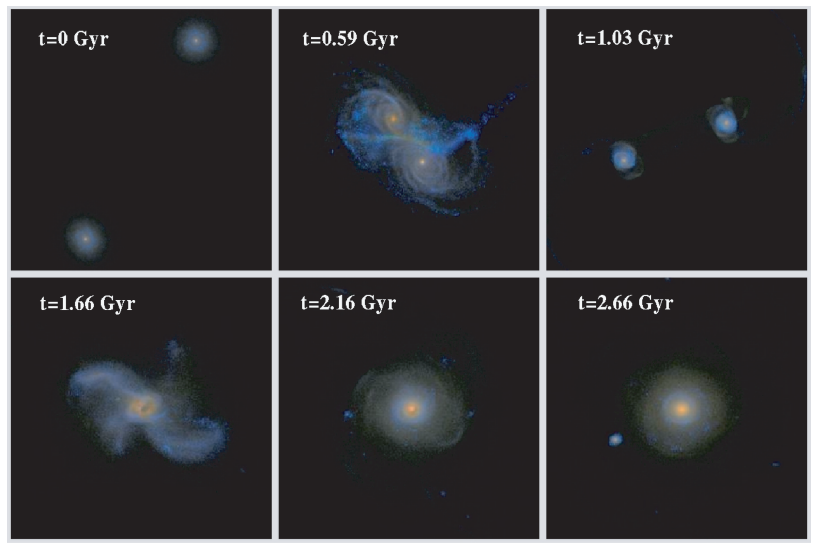
\includegraphics[width=0.4\textwidth]{Galaxy_Merger_J.M.Lotz.png}
    \caption{A look at how the time scale affects the shape of merging galaxies. Photo of simulation of equal-mass gas-rich disc merger. \citet{hopkins08}.}
    \label{fig:morphology}
\end{figure}

The current understanding of galaxy evolution is that major mergers between spiral galaxies are the primary way elliptical galaxies are created. A general picture is that once the galaxies are in gravitational range, tidal interactions happen that throw stars into random orbits, and this creates tails and bulges. Gravity pulls the center of the two galaxies together in a spring-like fashion until the centers are merged. Since the stars have taken on random orbits they create a giant spherical cloud around the center of mass, or an elliptical galaxy. Sometimes the galaxy shape is elongated or triaxial, meaning that there are still substructures present from the original disks. Formed structures also depend on whether it was a dry merger (galaxies with little gas) or a wet merger (gas-rich galaxies). With a gas-rich galaxy star formation can begin and new structures can be created.  

Despite the progress in understanding mergers, several questions remain regarding the final morphology of the MW-M31 merger. Will the remnant for a classical Hubble classification elliptical galaxy (E0-E7)? Will the galaxy exhibit elongations or triaxial characteristics? How does the shape vary as a function of the radius? Would the inner region act more spherical while the outer region shows underlying structures from the parent galaxies? Furthermore, would this merger be classified as wet or dry, and how does the remnant behave in terms of star formation? This paper focuses on the question of what shape the remnant takes, whether it is a traditional classification, and how the shape varies by radius. By addressing this question the project will help contribute understanding of mergers and how they reshape galactic structures. 

\section{Proposal}

\subsection{This Proposal}
This research aims to determine whether the MW-M31 merger remnant is a spheroid or exhibits elongation/triaxiality. Additionally, I will classify its Hubble type (E0, E7, S0) based on its shape and analyze whether its morphology varies with radius. 

\subsection{Methods}
I will use the van der Marel et al. (2012) simulation snapshots post-merger to analyze the stellar component of the remnant. I'll want to run a simulation with current stellar data points from the MW-M31 (not halo or dark matter), then analyze snapshots that happen when the simulation reaches equilibrium, probably a few Gyrs. The flow of work will be as follows: 

\subsubsection{Identify Relevant Snapshots and Particles}
\begin{itemize}
    \item Use the MW and M31 data sets provided in class
    \item ReadFile.py to load simulation
    \item GalaxyMass.py to get total mass of particle type (stellar for this project)
\end{itemize}

\subsubsection{Centering and Aligning the Remnant}
\begin{itemize}
    \item Determine COM position and velocity using CenterofMass.py
    \[
\mathbf{r}_{\text{COM}} = \frac{\sum m_i \mathbf{r}_i}{\sum m_i}
\]
    \item Run OrbitCOM.py to generate time simulation of merger, get snapshots of a few Gyrs
    \item Align the total angular momentum vector (\(\mathbf{L}\)) with the z-axis to view galaxy face on or edge on (Lab 7)
  \[
  \mathbf{L} = \sum_i m_i (\mathbf{r}_i \times \mathbf{v}_i)
  \]
\end{itemize}

\subsubsection{Visualizing Shape of Remnant}
Generate various plots to see the structure of the merged galaxy, snapshots should be aged a few Gyrs. 
\begin{itemize}
    \item Disk Density Plot both edge-on and face-on by using 2D histograms.
    \[
    \Sigma(R) = \frac{\sum m_i}{A}
    \]
    where \( \Sigma(R) \) is the surface density at radius \( R \), \( m_i \) are the masses of the particles, and \( A \) is the area of the bin.
    
    \item Velocity scatter plot both edge-on and face-on to see if there are any patterns in rotation.
    \[
    v_{\text{tan}} = \arctan\left(\frac{v_y}{v_x}\right)
    \]
    where \( v_{\text{tan}} \) is the tangential velocity derived from the velocity components.

    \item Plot radial distribution of stars to see how density of stars vary with radius. Recognize if shape is spherical, triaxial, elongated, has tidal tails, or spiral arms.
    \[
    \rho(r) = \frac{1}{4\pi r^2} \frac{dM}{dr}
    \]
    where \( \rho(r) \) is the density profile and \( \frac{dM}{dr} \) represents the mass enclosed in spherical shells.

    \item Plot radial velocity distribution to further distinguish between disk-like or elliptical structure.
    \[
    v_{\text{rad}} = \frac{x v_x + y v_y}{\sqrt{x^2 + y^2}}
    \]
    where \( v_{\text{rad}} \) represents the radial velocity component.

    \item Use MassProfile.py to compute the enclosed mass and circular velocity as a function of radius.
    \[
    v_{\text{circ}} = \sqrt{\frac{G M(r)}{r}}
    \]
    where \( v_{\text{circ}} \) is the circular velocity, \( G \) is the gravitational constant, and \( M(r) \) is the enclosed mass at radius \( r \).
\end{itemize}

\begin{figure}[h]
    \centering
    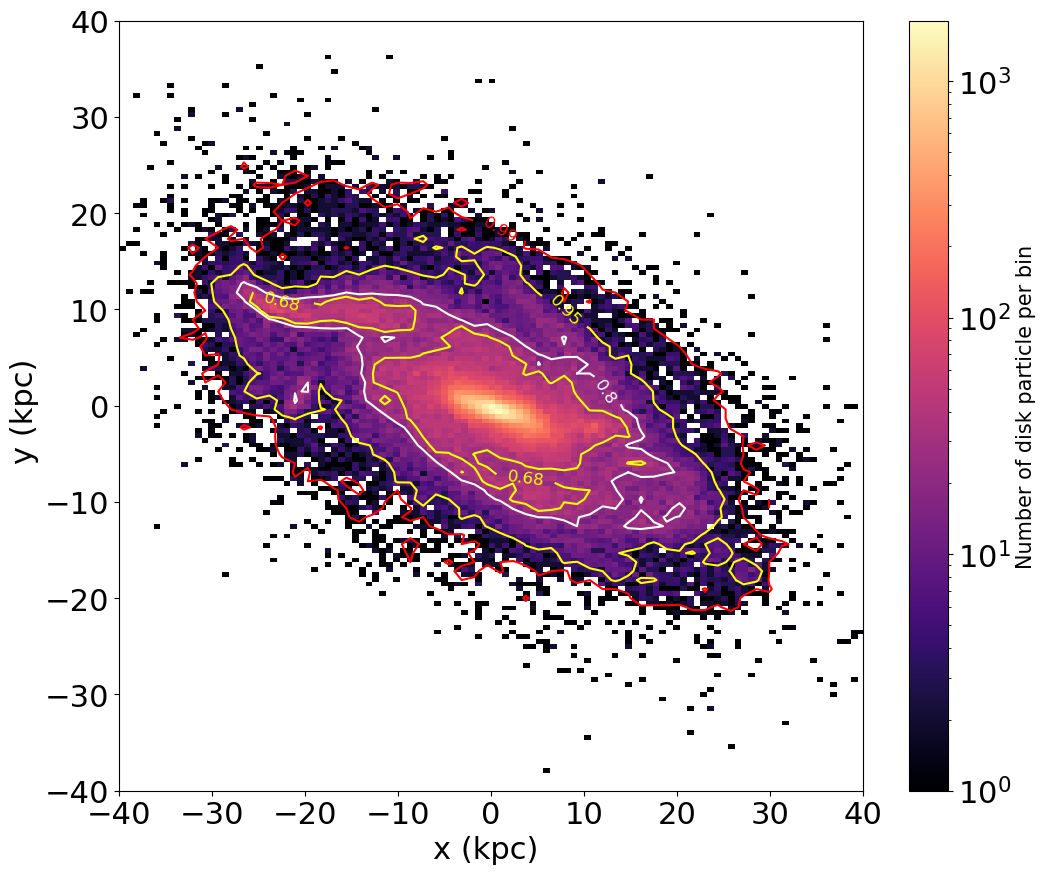
\includegraphics[width=0.4\textwidth]{Example Face On Density Plot.png}
    \caption{Methodology: example of a face on density plot of M31, generated in Lab7.}
    \label{fig:method}
\end{figure}

\subsection{Hypothesis}
My hypothesis is that the MW-M31 merger remnant will form a triaxial elliptical galaxy rather than a perfect spheroid. This is because both galaxy are large$1 \times 10^5$ ly
$2.6 \times 10^5$ ly, and are spiral galaxies with halos in the center on trajectory for a head on collision. I expect the center of the remnant to be rather spherical with the edges showing remnants of structure. 

\bibliographystyle{aasjournal}

\begin{thebibliography}{}
\bibitem[Barnes \& Hernquist(1992)]{barnes92} Barnes, J. E., \& Hernquist, L. E. 1992, ARA\&A, 30, 705
\bibitem[Lotz et al.(2008)]{lotz08} Lotz, J. M., et al. 2008, MNRAS, 391, 1137
\bibitem[Eliche-Moral et al.(2018)]{eliche18} Eliche-Moral, M. C., et al. 2018, A\&A, 617, A113
\bibitem[Van der Marel et al.(2012a)]{vandermarel12a} van der Marel, R. P., Besla, G., et al. 2012, 753
\end{thebibliography}


\end{document}
